%--------------------------------------------------------
% BEER PONG RULES: SETUP SECTION
%--------------------------------------------------------
\section{Setup}\label{sec:SETUP}

	\subsection{Cup Formation}\label{ssec:CupFormation}
		\subsubsection{} \label{sssec:CF,solocups}
			Each players rack is to be made up of 10 red 18 US-fluid-ounce solo cups.
            See Figure \ref{fig:solocup} for the regulation cup specifications.
		\subsubsection{}  \label{sssec:CF,triangle}
			The starting rack is a tight equilateral triangle with the base towards the player's table edge and the tip towards the opponent.
		\subsubsection{}  \label{sssec:CF,position}
			The rack's back edge is to be at least two finger widths from the edge but no more than 4 and centred from side to side.
		\subsubsection{}  \label{sssec:CF,kissing}
			Solo Cup rims must be "kissing". There should be minimal spaces in between the cups but not so close as to lean, tilt, or overlap onto their neighbouring cups.
			
	\begin{figure}[h]% Shows a single rack setup
		\centering
		\includegraphics[width=0.3\textwidth]{startingrack.png}
		\caption{Diagram of a full 10 rack of cups on a centred on the table. The arrow points towards the opponents rack. The hashed middle cup is the bitch cup (see \ref{ssec:BitchCup}).}
		\label{fig:therack}
	\end{figure}

	\subsection{Cup Content}\label{ssec:CupContent}
        \subsubsection{}\label{sssec:CC,filling}
            Cups are to be filled to a minimum that stops the moving and sliding when a ball is sunk into the cup.
        \subsubsection{} \label{sssec:CC,w_vs_l}
            The physical content of the cup is either water or liquor.
            \begin{enumerate}[label=(\alph*), leftmargin=2cm]
                \itemsep -1.25em 
                \item Water Cups: Water is put into the cups following Section \ref{sssec:CC,filling} regulations \\
                \item Drink Cups: Drinks are put into the solo cups following Section \ref{sssec:CC,filling} regulations and budget costs...
            \end{enumerate}
        \subsubsection{} \label{sssec:CC,rinse}
            A cup of water will be provieded to the players to rinse the balls off when playing with beer. This is for sanitary reasons.

    \subsection{The Balls}\label{ssec:Balls}
        \subsubsection{} \label{sssec:Balls,num}
            The game is played with 2, 1.57in or 40mm diameter, Ping Pong Balls. See Figure \ref{fig:solocup}
        \subsubsection{} \label{sssec:Balls,dents}
            The balls must have no dents.
        \subsubsection{}\label{sssec:Balls,bounce}
            The balls must be checked to have the same elasticity (bounce). 
        \subsubsection{}\label{sssec:Balls,texture}
            The texture of the balls must be consistent between the two; to the players standards. This is for consistency of throwing.

	\subsection{The Cup}\label{ssec:Cup}
			\subsubsection{}\label{sssec:Cup,dim}
				The solo cups are to be red, 18US-fluid-ounzes and have the dimensions as seen in Figure \ref{fig:solocup}.
			\subsubsection{}\label{sssec:Cup,broken}
				Cups should not be used if broken or cracked in any way. Change this cup out.
            \subsubsection{}\label{ssec:Cup,rinsing}
                Cups should be rinsed before a game in both water and drink versions before play. Cups can get quite gross.

    \begin{figure}
        \centering
        \includegraphics[width=0.9\textwidth]{dimensions.png}
        \caption{Dimensions of an regulation 18oz Solo Cup and Regulation ping pong ball.}
        \label{fig:solocup}
    \end{figure}
			
	\subsection{Teams}\label{ssec:Teams}
		\subsubsection{}\label{sssec:teams,options}
			There are two options to play beer pong: single or doubles.
            \begin{enumerate}[label=(\alph*), leftmargin=2cm]% Singles vs doubles
                \itemsep -1.25em 
                \item \textbf{Singles:} Beer pong can played as singles where for each rack there is one player.
                        This player will throw two balls each go (see Appendix \ref{app:A}).
                        The two balls (first and second throw) are independent for rules such as `on fire` and the `bounce`.\\
                \item \textbf{Doubles:}	This is a variation still played with two ping pong balls where each member of the team now throws a single ball.
                        Again, each ball is considered a independent for rules such as `on fire` and the `bounce` but this time it is by player and not throw order.
            \end{enumerate}
		\subsubsection{}\label{sssec:teams,choosing}
			There are no set rules for how teams are formed. Figure it out bud.
			
	\subsection{The Table}\label{ssec:Table}
		\subsubsection{}\label{sssec:Table,sides}
            The table is split into two sides down the midline (see Figure \ref{fig:table}).
			The opponents take opposite sides of the table long ways. 
			From the midpoint on the table in the direction the player is considered "their side"
		\subsubsection{}\label{sssec:Table,switch}
			If multiple games in a row are being played by the same players, they must switch sides every game.
		\subsubsection{}\label{sssec:Table,length}
			The table must be at least 5ft long.

    \begin{figure}
        \centering
        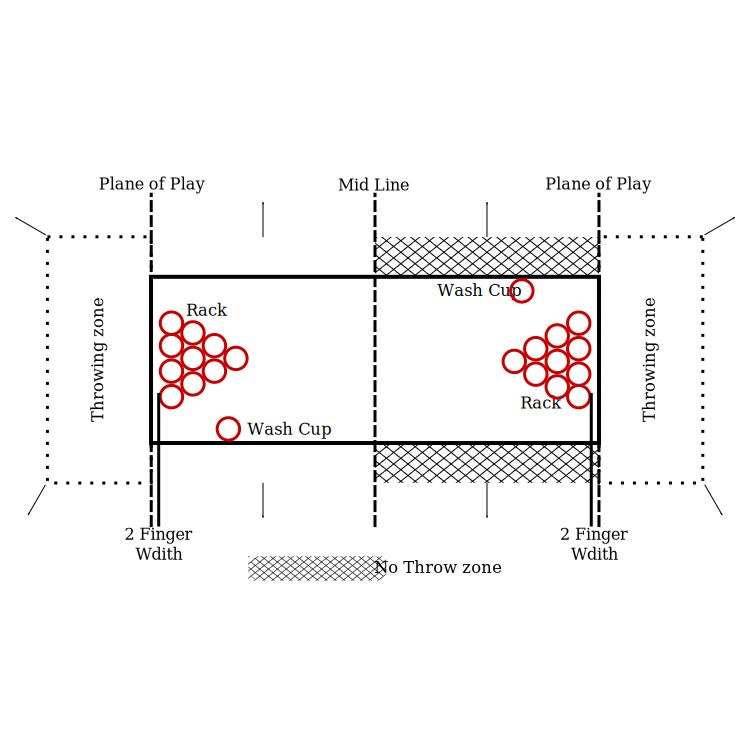
\includegraphics[width=\textwidth]{table.png}
        \caption{The table viewed from the top showing two racks, accepted throwing zones, the midpoint, and the 2 fingers from the edge that the rack has to be.}
        \label{fig:table}
    \end{figure}
